\chapter{Implementation And Testing}\label{impl_test}

		


	\section{Rectangles and Triangles Extraction Algorithm} 	
	

	%\section{} 	

	\section{Testing}
\begin{comment}

	As it can be seen in the picture, the software is logically divided in the four main components introduced in the design chapter (see \ref{chDesign}).
%, respecting the in the design specifics described in chapter \ref{chDesign}. 
	Both the feature extraction part and the class hierarchy respect the design specifications, described in such chapter. The classes responsible for the communication with \mbox{ACT-R} and the utility part.
The communication with  and


	\newpage
	
	\begin{sidewaysfigure}[hbtp]
	   \thispagestyle{empty}	
 	   \centering
	   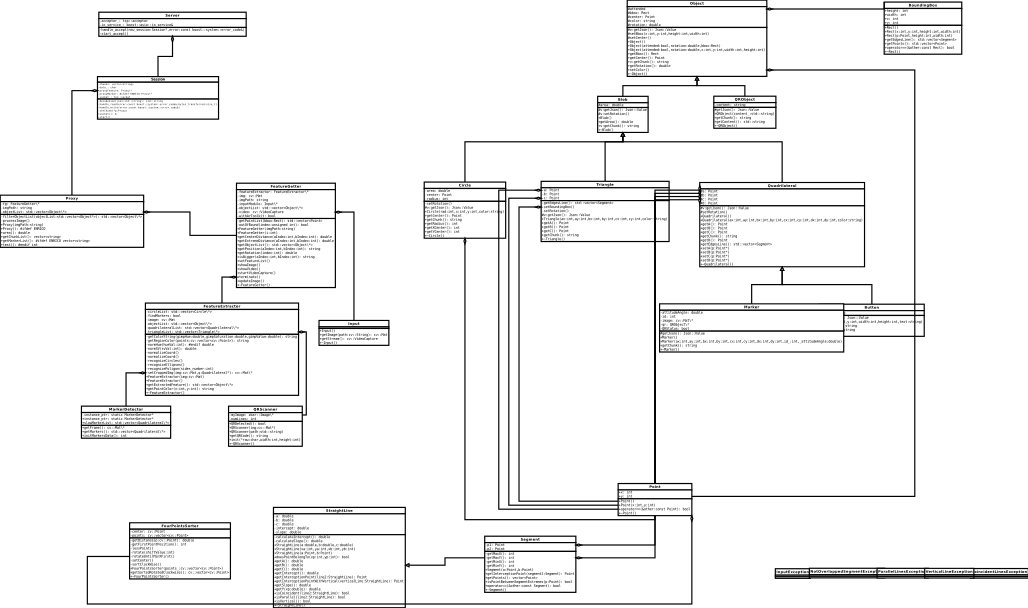
\includegraphics[height=\textheight]{images/ch_06/implementation.jpg}
	   
	  \caption{\textit{Class diagram illustrating the class hierarchy of the recognized objects}}  
	  \label{fig:HierarchyDesign}
 	\end{sidewaysfigure}

\newpage

\relax
	\AddToShipoutPicture*{ \\ \relax
	  \setlength{\unitlength}{1mm} 
	  \put(<10>, <10>){  
	    \makebox(0,0){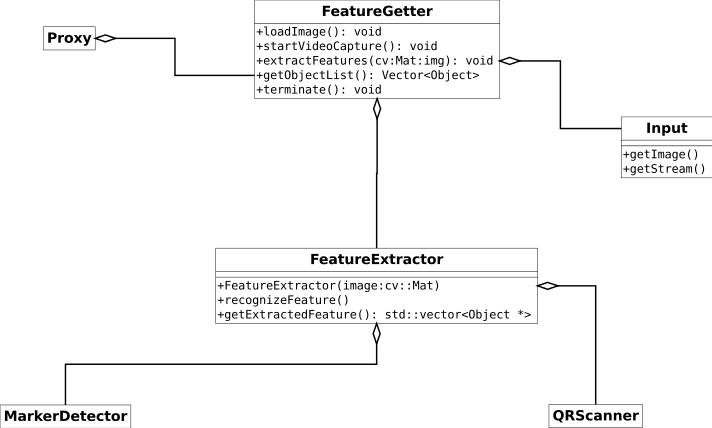
\includegraphics{images/ch_05/feature.png}}}} 
	ciao

	
\end{comment}

	%\section{COmmunication with ACT-R}
	%ciao
